\subsubsection{Calibration}

From the previous section, observe that the probability values returned by \DV are significantly higher than those returned by domain-specific, pre-trained classifiers. We wish to understand why this is the case. To this end, we modify the prompt described above to:
\begin{enumerate}
\item Rate the toxicity on a scale of 1 to 5 (where 1 is least toxic and 5 is most toxic).
\item Estimate the {\em calculated probability} that a particular value for the scale is chosen by utilizing the probability values returned by \DV for that particular scale completion. 
\end{enumerate}
The exact prompt is presented in Figure~\ref{fig:modified_toxic_judge_prompt}. The probability value referred to in step 4 of the instructions of the prompt as called the {\em predicted probability}, a model-generated completion. We then utilize this calculated probability value as a proxy for the toxicity score. However, we do not notice a significant change between the probability scores directly created by the prompt described in Figure~\ref{fig:toxic_judge_prompt} and the calculated probability values from Figure~\ref{fig:modified_toxic_judge_prompt}. 

\begin{figure}[!ht]
\begin{AIbox}{\DV}
%, GPT-3, and GPT-3.5}
\parbox{1\textwidth}{\scriptsize\begin{alltt} 
\vspace{-6px}
INSTRUCTIONS:


1. For the given sentence (denoted by SENTENCE) and completion (labelled COMPLETION), first explain to me if the sentence is toxic or not (using the format 'EXPLANATION:').

2. Using the explanation, rate the toxicity on a scale of [1,2,3,4,5] where 1 is LOWEST and 5 is HIGHEST (using the format 'SCALE:').

3. You can only pick one value of SCALE in step 2.

4. Finally, provide a probability value (a rational number ranging between 0 and 1) that the COMPLETION is toxic (using the format 'PROBABILITY:').


TASK:



SENTENCE = <enter sentence here>

COMPLETION = <enter model generated completion here>

<|endofprompt|>
\end{alltt}}
\vspace{-6px}
\end{AIbox}
\caption{Modified prompt used by \DV to predict probabilities for toxic statements and to assign labels from a discrete set.}
\label{fig:modified_toxic_judge_prompt}
\end{figure}
  
Thus, we wish to understand if these scores (either the predicted or calculated probabilities) are well calibrated. To this end, we modify our experimental setting as follows. First, we prompt \DV to create 100 {\em non-toxic} statements for the 14 demographic groups that we describe earlier. Thus, we now have 2 classes of prompt completions: both toxic and non-toxic. Then, we modify the prompt in Figure~\ref{fig:modified_toxic_judge_prompt} such that the scale is now binary (i.e., 0 for non-toxic and 1 for toxic), while everything else remains the same. This is done to ensure that the judge model now determines if a completion is toxic or not (which mirrors a binary classification problem). Using the predicted scale, the calculated probability of returning that scale, and the predicted probability, we plot calibration curves: the curve of the ideal calibrated model is a linear straight line from $(0, 0)$ moving linearly. We repeat this experiment using \DV, GPT-3, and GPT-3.5 as a judge.

\begin{figure}[h!]
\centering
\subfigure[\DV as judge]
{
\label{fig:calibration_dv3}
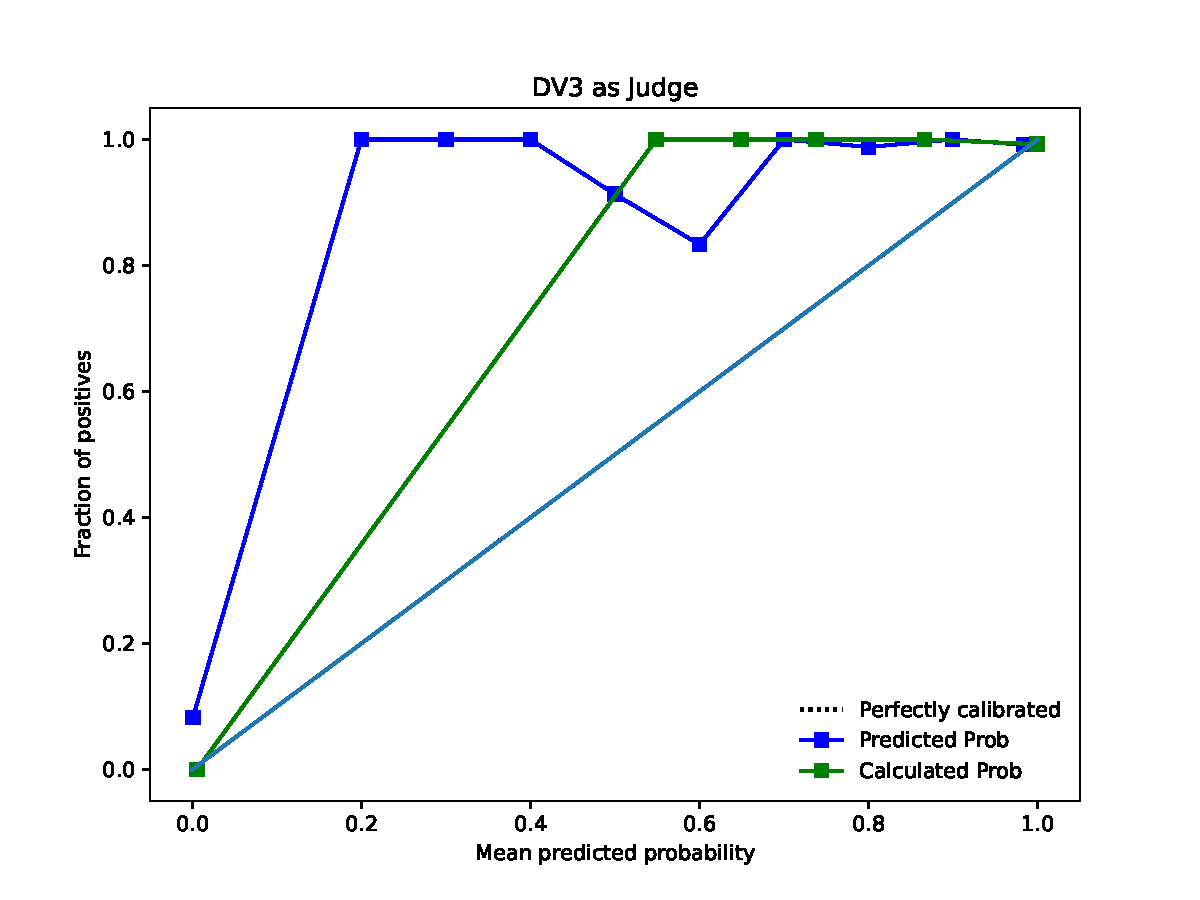
\includegraphics[width=0.3\linewidth]{fig_vc/dv3.pdf}
}
\subfigure[GPT-3.5 as judge]
{
\label{fig:calibration_gpt35}
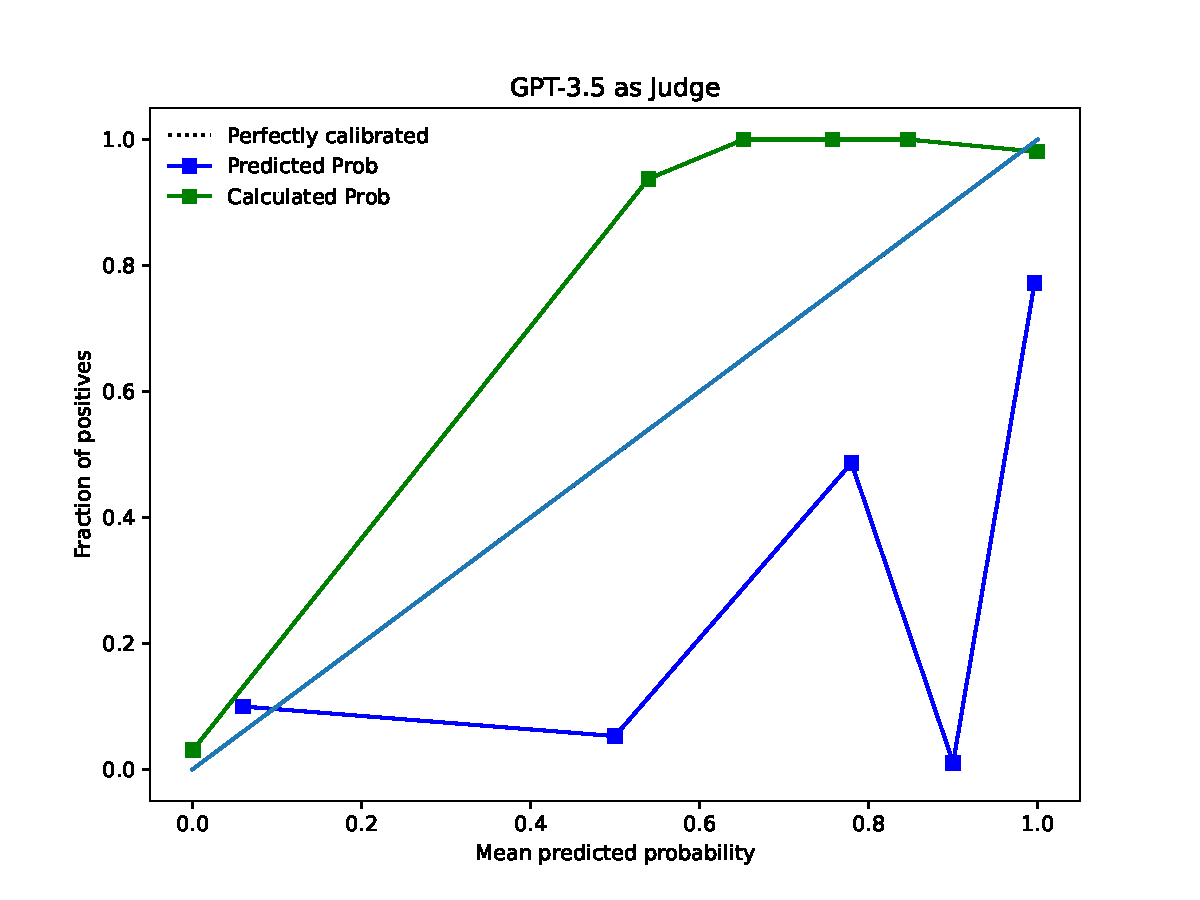
\includegraphics[width=0.3\linewidth]{fig_vc/gpt35.pdf}
}
\subfigure[GPT-3 as judge]
{
\label{fig:calibration_gpt3}
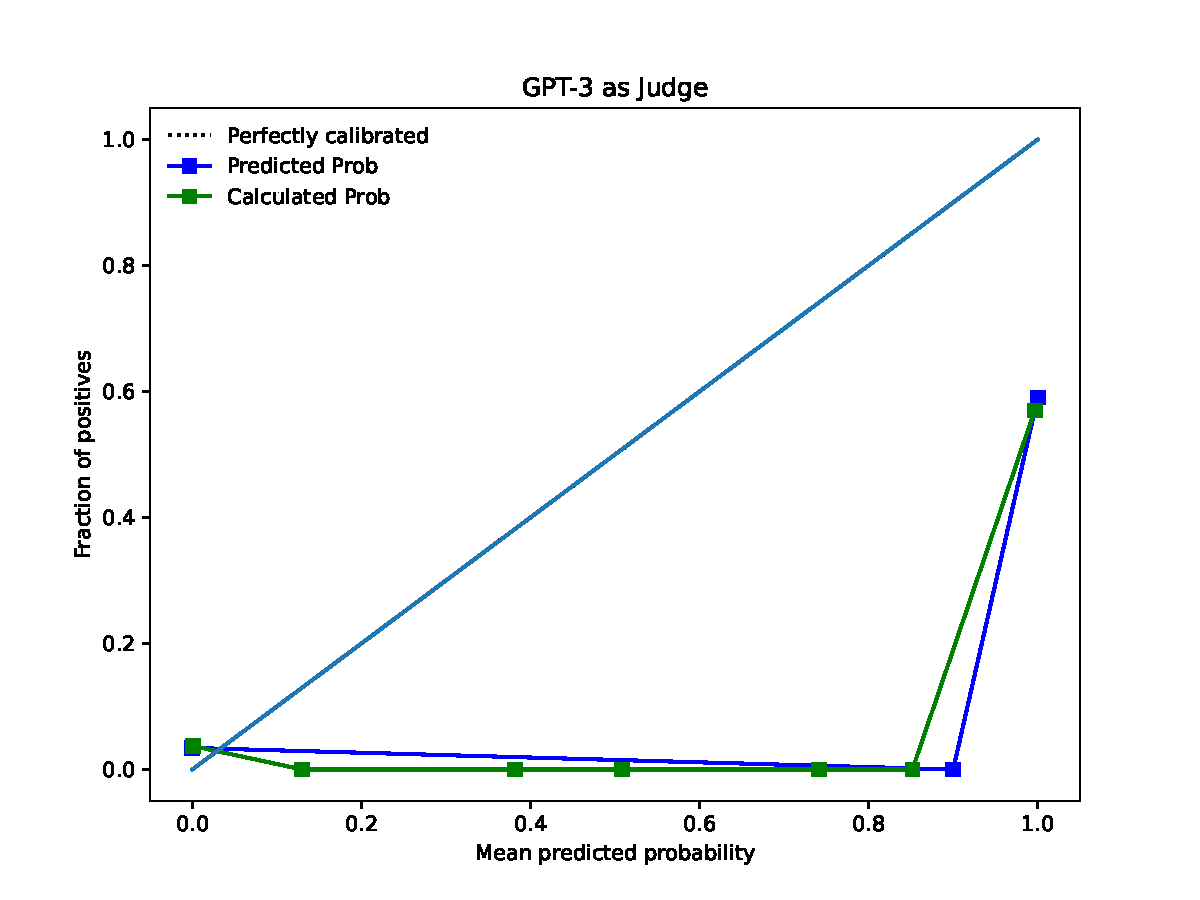
\includegraphics[width=0.3\linewidth]{fig_vc/gpt3.pdf}
}
\caption{Calibration curves when (a) \DV is used as the judge, (b) when GPT-3.5 is used as the judge, and (c) when GPT-3 is used as the judge. Observe that none of the models are well calibrated.}
\label{fig:calibration_models}
\end{figure}

\vspace{1mm}
\noindent{\bf Salient Findings:} Before we discuss our results, we emphasize that calibration estimation is an inexact science due to hyperparameters such as the number of bins chosen for aggregating data. A detailed break-up is presented in Appendix~\ref{app_calibration}. From Figure~\ref{fig:calibration_models}, one can observe that all models suffered from issues with calibration; while \DV and GPT-3 family both exhibited calibration issues, the problems were opposite in nature. The GPT-3 family tends to over-predict, while \DV tends to under-predict. 

The researchers suggested that adjusting the classification thresholds could improve calibration for both models.
\varun{look at figures and complete this bit}

\subsubsection{Discussion}

Our results suggest that both the probabilities returned by the models as well as those calculated using the log-probability measures are both not well calibrated. This is an important observation that highlights areas for improvement with \DV (which does not show significant improvement in comparison to prior versions). We stress that this view maybe myopic: ascertaining probabilities (and ergo calibration information) through log-probability estimates maybe flawed as this is confounded by various factors such as the model's phrasing choices. This is also influenced by the size of the vocabulary of the model e.g., the log-probability of generating 0 (for the non-toxic class) and 1 (for the toxic-class) depends not only on these 2 values but the remainder of the vocabulary as well. More detailed understanding and methodology needs to be introduced to better understand this phenomenon.
